\subsection{级数}

考虑豪斯多夫交换群中的点列 \((x_{n})_{n\in \mathbb{N}}\)，并作部分和序列 \(s_n = \sum_{p=0}^{n} x_p (n \in \mathbb{N})\)。映射 \((x_{n}) \to (s_{n})\) 是集合 \(\mathbf{G}^{\mathbf{N}}\)（即点列 \((x_{n})\)（\(\mathbf{G}\) 中的）的全体）到其自身上的双射；因为若给定了序列 \((s_{n})\)，则序列 \((x_{n})\) 由关系 \(x_{0} = s_{0}, x_{n} = s_{n}-s_{n-1} (n \geqslant 1)\) 确定。

由序列 \((x_{n})\) 所定义的级数，或通项为 \(x_{n}\) 的级数{[}在不致混淆时，按用语之便，径称级数 \((x_{n})\){]}，定义为如上相关联的序列偶 \((x_{n})\) 与 \((s_{n})\)。由序列 \((x_{n})\) 所定义的级数称为收敛的，如果序列 \((s_n)\) 收敛；这个序列的极限称为级数的和，记作 \(\sum_{n=0}^{\infty} x_n\)（按记号之便，或记 \(\sum_{n=0}^{\infty} x_n\)）。

若通项为 \(x_{n}\) 的级数收敛，我们有时会按用语之便，称它为“级数 \(\sum_{n=0}^{\infty} x_{n}\)”或“级数 \(x_{0} + x_{1} + \cdots + x_{n} + \cdots\)”。

通项为 \(x_{n}\) 的级数收敛的一个必要条件是序列 \((s_{n})\) 为 Cauchy 序列，也就是说，对 G 中原点的每个邻域 V，存在整数 \(n_{0}\)，使得对每对整数 \(n \geqslant n_{0}, p > 0\)，有

\[
s _ {n + p} - s _ {n} = \sum_ {i = n + 1} ^ {n + p} x _ {i} \in V.
\]

若 \(\mathbf{G}\) 是完备的，这个条件也是充分的（级数的 Cauchy 判别准则）。

若通项为 \(x_{n}\) 的级数收敛，特别地我们有 \(\lim_{n\to \infty}(s_n - s_{n-1}) = \lim_{n\to \infty}x_n = 0\)；但这个收敛的必要条件一般绝不是充分的，即使 \(G\) 是完备的也是如此（见第四章，§ 7）。

命题 7. 若由序列 \((x_{n})\) 与 \((y_{n})\) 所定义的级数都收敛，则由序列 \((-x_{n})\) 与 \((x_{n} + y_{n})\) 所定义的级数也收敛，并且我们有

\[
\sum_ {n = 0} ^ {\infty} (- x _ {n}) = - \sum_ {n = 0} ^ {\infty} x _ {n},\tag{7}
\]

\[
\sum_ {n = 0} ^ {\infty} \left(x _ {n} + y _ {n}\right) = \sum_ {n = 0} ^ {\infty} x _ {n} + \sum_ {n = 0} ^ {\infty} y _ {n}.\tag{8}
\]

这是 \(-x\) 在 \(\mathbf{G}\) 上连续以及 \(x + y\) 在 \(\mathbf{G} \times \mathbf{G}\) 上连续的一个明显推论。

推论. 若 \((x_{n})\)、\((y_{n})\) 是 G 的两个点序列，使得除有限个指标外都有 \(x_{n}=y_{n}\)，且通项为 \(x_{n}\) 的级数收敛，则通项为 \(y_{n}\) 的级数也收敛。

因为通项为 \(x_{n} - y_{n}\) 的级数从某个指标起各项皆为零。

这个推论可以表述为：我们可以任意改动收敛级数的有限个项而不使它失去收敛性。特别地，若 \(y_{n} = 0\)（对 \(n < m\)），且 \(y_{n} = x_{n}\)（对 \(n \geqslant m\)），

则我们看到通项为 \(y_{n}\) 的级数收敛当且仅当通项为 \(x_{n}\) 的级数收敛；其和记作 \(\sum_{n=m}^{\infty} x_{n}\)，称为指标为 \(m\) 的余项（级数 \((x_{n})\) 的余项）。由于

\[
\sum_ {n = m} ^ {\infty} x _ {n} = \sum_ {n = 0} ^ {\infty} x _ {n} - s _ {m - 1},
\]

收敛级数的第 \(m\) 余项当 \(m\) 趋于 \(+\infty\) 时趋于 o。

若序列 \((x_{n})_{n\in I}\) 的指标集是 \(I\)——\(N\) 的无限子集——，且 \(\varphi\) 表示 \(N\) 到 \(I\) 上的保持严格序的双射，则按用语之便，称由序列 \((x_{\varphi(n)})_{n\in N}\) 所定义的级数为由序列 \((x_{n})_{n\in I}\) 所定义的级数；若这个级数收敛，其和记作 \(\sum_{n\in I}x_n\)。立即可以验证，这个级数收敛当且仅当通项为 \((z_n)\) 的级数收敛，其中 \(z_{n}=x_{n}\)（若 \(n\in I\)），而 \(z_{n}=0\)（若 \(n\in G I\)）。

\pandocbounded{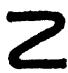
\includegraphics[keepaspectratio]{images/part002_ebf593f8.jpg}}

值得注意的是，若由序列 \((x_{n})_{n\in \mathbb{N}}\) 所定义的级数收敛，仍可能存在 \(\mathbf{N}\) 的无限子集 I，使得由子列 \((x_{n})_{n\in \mathbb{I}}\) 所定义的级数不收敛（见习题 5 及第四章，§ 7）。

命题 4 与命题 5 立即推广到级数，我们把它们在这一情形的表述留给读者。

命题 8（级数的受限结合性）. 设 \((k_n)\) 是一个严格递增的整数序列（\(\geqslant 0\)）。若通项为 \(x_n\) 的级数收敛，且令 \(u_n = \sum_{p=k_{n-1}}^{k_n-1} x_p\)，则通项为 \(u_n\) 的级数收敛，且我们有 \(\sum_{n=0}^{\infty} u_n = \sum_{n=0}^{\infty} x_n\)。

因为级数 \((u_{n})\) 的部分和序列是一个子列 \((s_{k_{n}-1})\)，它取自部分和序列 \((s_{n})\)（级数 \((x_{n})\) 的部分和序列）。

